\documentclass[authoryear]{elsarticle}
\usepackage{tabulary}
\usepackage{eurosym}

\makeatletter
\g@addto@macro\@floatboxreset\centering
\makeatother

\begin{document}

\title{A History of Downtown Congestion Pricing}
\author[ll]{Lewis Lehe \corref{cor1}}

\address[ll]{UC Berkeley, Department of Civil and Environmental Engineering \\ lewis500@berkeley.edu \\ http://lewislehe.com}

\begin{abstract}

``Downtown congestion pricing'' (DCP) is what this paper calls the practice of charging tolls on driving in a city's central areas in such a way as to relieve traffic congestion. Five major cities have implemented DCP: Singapore, London, Stockholm, Milan and Gothenburg. Of these, Singapore and Milan have implemented two schemes. This paper reviews the history of DCP from the 1950's to the present-day, reporting on each system's implementation, design, transportation impacts and finances as well as providing some outside historical developments. Along the way, two themes recur: First, that exemptions from charging are highly consequential, as exempt traffic quickly grows after tolls are put in place. Second, that instituting a toll discourages much more traffic than increasing one does. Plans for the future are also noted. 

\end{abstract}

\maketitle

\section{Introduction}

Today, authorities in Vancouver and New York City are considering implementing tolls on zones of their downtown street networks as a means of relieving traffic congestion---a practice we will call ``downtown congestion pricing'' (DCP). Forms of congestion pricing are already in place on highways and bridges throughout North America, such as Highway 407 in Toronto and the High-Occupancy Toll (or ``Express'') Lanes now proliferating across the United States. But the schemes being considered for New York City and Vancouver would differ from not only by their setting but also topologically: while congestion pricing on highways charges drivers to travel between well-defined start and end points, DCP charges for use of  clusters of contiguous downtown streets (``zones''); charged trips can thus begin and end at numerous points within the zone or along its boundary. Thus, DCP is attended by administrative and technological concerns that warrant special treatment.

To date, only five cities have implented DCP as we have defined it: Singapore, London, Stockholm, Gothenburg and Milan. This paper provides a broad sweep of their experiences along with some historical connective tissue. The goal is to help the reader quickly become familiar with the experience of DCP thus far and to point toward works containing further information. Similarly, \citet{Hau1992}, \citet{Gomez-Ibanez1994}, \citet{Small1998} and \citet{Anas2011} survey various congestion pricing schemes up to their publications, with \citet{Gomez-Ibanez1994} being especially thorough, but this paper includes later developments and emphasizes the special concerns of downtown schemes.

\subsection{Organization and scope}

We describe six DCP schemes: Singapore's Area License Scheme (\ref{sec:als}), Singapore's Electronic Road Pricing (Sec. \ref{sec:erp}), the London Congestion Charge (Sec. \ref{sec:london}), the Stockholm Congestion Tax (Sec. \ref{sec:stockholm}), Milan's Ecopass and Area C\footnote{These are treated together as Area C is technologically the same as Ecopass but has different prices and exemptions.} (Sec. \ref{sec:milan}) and the Gothenburg Congestion Tax (Sec. \ref{sec:gothenburg}). Each description includes four subsections:

\begin{enumerate}
    \item \emph{Implementation}. Motivation and events leading up to implementation.
    \item \emph{Design}. The scheme's technology, prices, exemptions and geography---including changes over time.\footnote{In these sections, details about scheme design comes from the schemes' official websites except when otherwise noted.}
    \item \emph{Transportation Impacts}. Impact on travel---especially on the magnitude and composition of flow into the charged zone and, where available, on speeds and transit ridership. Note that DCP also affects air pollution, equity, real estate and commerce. But the transportation impacts are the most well documented, comparable and, arguably, \emph{direct} impacts. The reader interested in other effects---which are undoubtedly important---can usually find such information in the works cited.
    \item \emph{Finances}. How much money the scheme has cost to build and operate, and how much revenue it has raised.
\end{enumerate}

In between are sections devoted to historical context. Sec. \ref{sec:early} describes intelletual developments prior to real implementation. Sec. \ref{sec:transition} describes a twenty-year ``transition period'' following Singapore's first scheme. Sec. \ref{sec:future} briefly describes future plans. 

Note that, for brevity and focus, certain developments in the history of DCP have been omitted. For example, Valetta, Malta \citep{Attard2010} and Durham, England \citep[p.269]{Santos2006a} also apply tolls to central areas, but these schemes are very small and not much data is collected on their outcomes. 

% Likewise, about ten schemes were proposed but languished or been cancelled (including Hong Kong, Edinburgh, Manchester, New York City, San Francisco, Cambridge, the Randstadt region of the Netherlands and Helsinki), but among these only Hong Kong's is discussed, because it provides context for Singapore's ERP.

\subsection{Themes}\label{ssec:themes}

The paper is more focused on description than inference, but we do point out two recurring themes.

Theme I is that exemptions are among the most consequential aspects of a scheme's design, to a degree that often surprises authorities. Exempt classes of trips or vehicles quickly become a large share of traffic, and in doing so they compromise congestion goals and reduce revenue more than projected.

Theme II is that charging implementing a toll is much more consequential than differences in the toll level. When a scheme is implemented, entries to the tolled zone by vehicles subject to charge drop sharply, but later toll increases make only a minor difference. Noting this effect in Stockholm and Gothenburg, \citet[p. 45]{Borjesson2018} offer two explanations. The first is grounded in traditional economic theory: the initial toll discourages all the drivers with elastic demands, so the traffic exposed to later toll increases is composed of drivers with a high willingness-to-pay for travel. The second explanation is grounded in behavioral economics: \citet{Shampanier2007} note that consumers are extremely sensitive to being charged \emph{any} positive price---even negligible ones.


\section{Early steps}

The idea of DRP was first incubated from the mid 1950's until the early 1970's. The first such proposal seems to be \citet{buchanan1952}'s passing mention of a ``city license,'' an idea \citet{Walters1954} fleshes out in somewhat more detail: ``A special `London licence' would have to be acquired and displayed before vehicles could use the roads of central London between 8 a.m. and 6 p.m.'' But the first detailed proposal came in a 1959 testimony to the US Congress about traffic problems in Washington, D.C. by the economist William Vickrey \citep{Vickrey1959}. 

Vickrey proposed a system whereby the the Washington, D.C. metropolitan area would be divided into zones (``between 60 and 200''). Drivers would be charged a time-varying toll whenever they crossed one of the zone boundaries. For enforcement, Vickrey proposed an instance of what \citet{DePalma2011} call a ``tag and beacon'' system, which is now most commonly used on toll roads and bridges. In such a system, toll sites have a ``beacon'' located over, beside or under the roadway, which constantly emits electromagnetic waves  (e.g., radio or microwave). Vehicles carry a ``tag'' which, when struck by these waves,  fires back an identifier code. A central system then tallies a charge against the account or vehicle-owner associated. Remarkably, Vickrey actually demonstrated the transponder apparatus for Congress using a model train .\footnote{Richard Arnott and Marvin Krauss later cleaned up Vickrey's testimony and published it as \citet{Vickrey1994}.} Nothing, however, directly came of Vickrey's scheme.

While Vickrey was at work on Washington's problems, British officials perceived a traffic crisis: the number of registered vehicles had doubled in the 1950's, but expenditure on roads was low and British towns had ancient street layouts \citep[p.523-524]{Gunn2011}. To deal with urban congestion, the Ministry of Transport comissioned several reports. One, the ``Buchanan Report'' (CITE) recommended planning solutions and city reconstruction. The other, the ``Smeed Report'' \citep{MoT1964}, set out principles and proposes schemes of varying levels of technical complexity. But ultimately, it was the Buchanan Report that wound up influencing the government more in the short term.\footnote{See \citep{Rooney2014} for an account of the conflict between the planning and pricing approaches.}

MAKE SOME CONCLUDING STATEMENT


\section{Singapore Area License Scheme}

\subsection{History}

In the early 1970's, Singapore took an interest in downtown pricing for the same reason Britain had ten years earlier: quick growth in car ownership. Between 1960 and 1970, the private vehicle population doubled as the country grew wealthier and built residential estates in its hinterlands, but the length of public roads rose only 35\% \citep[p.211-212]{Santos2004}. The government responded forcefully by consolidating bus operators, a six-fold increase in road spending from 1975 to 1980, plans for a metro and high taxes on car ownership\footnote{See Appendix B of \citet{Gomez-Ibanez1994} for a list of Singapore's policies against car ownership.} \citep{Santos2004}. 

In 1973, the government convened the Road Transport Action Committee (RTAC) to tackle downtown congestion. The Committee's first proposals included bus lanes as well as efforts to encourage staggered work hours (especially for public employees) and carpooling \citep{Chin1998}. In May 1974 the RTAC published a report declaring, ``Singapore cannot afford to continue to allocate scarce and valuable land to build unlimited miles of roads'' \citep[p.3]{SRTAC1974}. The plan proposed four policies: (i) sharp increases in CBD parking rates; (ii) new commuter bus services; (iii) a park-and-ride scheme whereby commuters would park in garages outside the CBD and take special shuttles to their workplaces; (iv) the Area License Scheme---a simple supplementary license system that made up the core of the plan.\footnote{It is possible the idea for ALS came when Gabriel Roth (of the Smeed committee), who was then working in Singapore as a consultant for the World Bank, passed the World Bank's plan for road pricing in Caracas, \citet{Vorhees1973}, to members of the RTAC (CITE ROTH 1996).} ALS commenced on June 3, 1975 and continued until 1998. 

\subsection{Design}

At shops and roadside booths, drivers paid S\$3 to buy a daily ``license'', or S\$60 for a monthly one, that permitted them to enter to a 6.2 km$^{2}$ Restricted Zone (RZ), Monday through Saturday morning \citep{WatsonHolland1978}. The ``license'' was a paper decal that went in the windshield. Wardens standing by the road at 22 access points to the RZ wrote down the plate numbers of vehicles lacking licenses. At first, only private vehicles with fewer than three passengers had to show licenses. Taxis, commercial goods vehicles, public vehicles, motorcycles, carpools and buses were exempt, but taxis lost their exemption within three weeks. While the charging period was 7:30-9:30 AM originally, authorities  extended charging to 10:15 AM on August 1. The Park-and-Ride scheme was essentially shut down within a few months for lack of ridership, and the new bus services did not draw many customers. 

There were many changes to ALS over the years.\footnote{See Table 1 of \citet[p. 98]{PhangToh1997} for a table listing changes. } In 1976, the price of a license was increased to S\$4 and a double rate charged to registered company cars, because firms could deduct the charge from taxes. In 1977, charges for taxis were cut to S\$2. In 1980, the license price rose to S\$5 (S\$10 for company cars). Throughout the 1980s, the boundaries of the RZ were expanded to enclose new developments. In 1989, carpools, goods vehicles and motorcycles lost their exempt status, and an evening charging period was added.\footnote{Note that the evening period was not an outbound charge, and a single license purchased travel in both periods.} In January 1994, a S\$2 license was added for entry from 10:15 AM to 4:30 PM \citep{PhangToh2004}. A vehicle entering the RZ in either or both peaks needed a Whole Day license (also good between the peaks), while a driver who entered only between the peaks only needed the Part Day license. 

Finally, while not technically part of ALS, in June 1995 the government implemented a parallel system called the Road Pricing Scheme (RPS) on one expressway. Drivers without a valid ALS license were required to buy a cheaper RPS license to drive there from 7:30-8:30 AM.

\subsection{Results}

Between March and October of 1975, vehicle entries to the RZ during the 7:30-10:15AM charging interval fell by 44\%---well beyond RTAC's desired 25-30\% reduction \citep{WatsonHolland1978}. Since the result exceeded expectations so drastically, some observers---including \citet{Wilson1988a,McCarthyTay1993} and \citet{WatsonHolland1978}---have concluded that initial charges were too high.

Speed results appear in Table \ref{tab:speed-singapore}. Commute trips into the RZ primarily switched to bus and carpool, while travelers who had traversed the RZ in the morning to destinations outside tended to switch to a ring road. 

A household survey of travel times conducted yielded disappointing results. There was almost no effect on traffic in the charge-free evening peak; and, due to the fall in speeds on the ring-road and mode shifting to slower modes such as bus and carpool, average journey times worsened in the short term. 

\begin{table}[ht]

\begin{tabular}{c>{\centering}p{3cm}>{\centering}p{3cm}}
 & before ALS\\
(kph estimated) & after ALS \\
(kph observed)\tabularnewline
\cline{2-3} 
Restricted Zone & 27 & 33\tabularnewline
\cline{2-3} 
inbound radials & 29 & 32\tabularnewline
\cline{2-3} 
outbound radials & 35 & 35\tabularnewline
\cline{2-3} 
ring road & 25 & 20\tabularnewline
\end{tabular}

\caption{Singapore speeds before and after Area License Scheme implementation \citep[p.10]{WatsonHolland1978} }
\label{tab:speed-singapore}
\end{table}

The 1989 reforms yielded major rebalancing of morning traffic flows: a rise and entries by car and taxi partly offset a roughly 50\% falls in entries by truck and motorcycle. In the new evening charging period, entries fell by 54\% and exits by 34\% \citep[p. 19]{Gomez-Ibanez1994}. Also, although less data are available for the 1994 introduction of the Part-Day pricing, traffic and congestion fell in the periods just after the morning and just before the evening period (CITE Phang et al., 1997).

\subsection{Finances}

ALS could be said to have the highest rate-of-return of any downtown pricing scheme. While the capital cost of implementation was S\$6.6 million, in fact 95 percent of that cost was sunk into the park-and-ride system \citet[p. 38]{WatsonHolland1978}. Initial revenues from license sales were S\$225,000 per month and operating costs were S\$50,000 per month. By 1993, annual revenues were S\$47 million, of which operating costs consumed 9 percent \citep{PhangToh2004}. In 1998, (just before the scheme ended) ALS and RPS earned about S\$100 million \citep{Chin2010}.
\section{A transition period}\label{sec:transition}

After ALS, no new DCP systems were launched until 1998, but there were several technological developments in the intervening years that paved the way for future schemes. This section describes two---Hong Kong's Electronic Road Pricing and the Norwegian toll rings---because of their scale and direct influence. But there were also  proposals drafted for DCP in other cities which never left the drawing board; see \citet{Gomez-Ibanez1994} and \citet{Small1998} for descriptions.

\subsection{Hong Kong Electronic Road Pricing}

 Between 1983 and 1985, Hong Kong conducted studies of a DCP system called ``Electronic Road Pricing'' (ERP). ERP was to be a tag-and-beacon system, wherein inductive loops embedded in the pavement at tolling sites---positioned to form cordons---would harvest ID's from transponders placed underneath vehicles \citep{Dawson1986}. Users received a monthly bill listing the price, place and times of all charging events. Field trials involving 2,500 equipped vehicles and 18 tolling sites showed the technology to be reliable. Meanwhile, modelling studies considered three main scenarios for the charging structure and topology \citep[Table 11, p. 23]{Gomez-Ibanez1994}. Tolling sites would be placed so as to divide Hong Kong into up to 13 zones with prices that varied by time-of-day and direction of travel. 

 Despite succesful tests and modelling that forecast large gains, Hong Kong did not adopt ERP when the study concluded. Many factors contributed \citep{Hau1990,Borins1988}, but two stand out. First, the trials ended exactly as outside developments (recession, new infrastructure, vehicle taxes) had mitigated congestion. Second, Britain was then negotiating to deliver Hong Kong to China in 1998, prompting worries about spying, and  ERP's monthly list of vehicle movements inflamed those concerns. Nontheless, although it was not implemented, the Hong Kong experience demonstrated the technical feasibility of wireless charging in a dense city, and its political failure influenced Singapore's choice of technology for its own ERP scheme.
 
\subsection{Norwegian Toll Rings}

Around 1990, the three largest Norwegian cities implemented ``toll rings,'' in which a cordon of tolling sites encloses an entire city. Bergen launched the first toll ring in January 1986 with six tolling sites on arterials leading into the city \citep{Ieromonachou2006,Ramjerdi2004,Gomez-Ibanez1994}. At each site, half the lanes had staffed toll booths and the other half were non-stop lanes reserved for cars displaying ``season pass'' stickers. Oslo opened its toll ring in January 1990 using a microwave tag-and-beacon system alongside tollbooths and coin payment lanes. In October 1991, Trondheim opened the third toll ring using the same electronic system as Oslo, but with tolls varying slightly over the day.

The toll rings are not examples of DRP as we have defined it; they are pure revenue devices with little intended or realized effect on traffic, due to their low prices and large cordons. What is novel about the toll rings is their business model:  governments in some region draw up a list of transportation projects, then incorporate a toll company whose revenues partly pay for these projects \citep{Ieromonachou2006}. Later, a similar model would motivate the adoption of the Stockholm and Gothenburg Congestion Taxes in nearby Sweden.


\section{Singapore --- Electronic Road Pricing (ERP)}

\subsection{History}

While cheap to administer, a manual system such as the Area License Scheme becomes intractable if authorities want to price precisely. For example, \citet[p. 4]{Chin2010} describes ALS once multiple charging periods and vehicle classes had been added: ``There were 16 different types of licences in use at its peak, and much concentration by the enforcement officers was required to ensure that they identified them correctly.''
To gain precision with less difficulty, in the early 1990s, Singapore solicited bids for an electronic system. The government chose a smart card/IU system like the one trialed in Cambridge, rather than a transponder system like the Hong Kong ERP, partly to alleviate privacy concerns \citep{PhangToh1997,Chin2010}. After extensive field trials and publicity, the electronic system---called, like Hong Kong's Electronic Road Pricing (ERP)---commenced operation in September 1998.

\subsection{Design}

\citet{Menon2004} describes ERP as having three components.

\begin{itemize}
\item In-vehicle Unit (IU), an electronic device that sits on vehicles' dashboards or handlebars and. The IU has a slot for a ``CashCard'' that the user can load up with money at various places.\footnote{The CashCard can also be used to pay for parking. In March 2015, a sevice called vCashCard was announced that allows drivers to pay with debit or credit without having a physical CashCard in the IU. (http://www.straitstimes.com/singapore/transport/virtual-cashcard-aims-to-solve-erp-woes)} There are IU's for each of six vehicle classes (see Figure \ref{fig:singapore-IUs}), because the toll charged to a vehicle is a multiple of its ``Passenger Car Unit'' (PCU), an index of how much roadspace the vehicle takes up (see Table \ref{tab:passenger-car-units}). 

\item Gantries (see Fig. \ref{fig:singapore-gantry}). Gantries are positioned in pairs. When a vehicle passes below, the first gantry signals the vehicle's IU, telling it to charge the CashCard appropriately. An optical sensor on the second gantry confirms the vehicle type matches the IU. In the event of error, a camera on the first gantry captures the rear number plate. 

\item The central control system, which verifies charges and issues notices and fines when there is a violation or error.
\end{itemize}

\begin{table}
	\begin{tabular}{|c|c|}
		\hline 
		PCU's & Vehicles\tabularnewline                              
		\hline 
		\hline 
		0.5   & motorcycles\tabularnewline                           
		\hline 
		1     & cars, taxis, light goods vehicles\tabularnewline     
		\hline 
		1.5   & heavy goods vehicles/small buses\tabularnewline      
		\hline 
		2     & very heavy goods vehicles/large buses\tabularnewline 
		\hline 
	\end{tabular}
	
	\caption{
	Passenger Car Units (PCU's) for ERP. Vehicle charges are weighted by the PCU number---e.g., a very heavy goods vehicle pays four times what a motorcycle does. \citep{LTA2016} 
	}
	\label{tab:passenger-car-units}
\end{table}

ERP varies tolls substantially by time-of-day. Figure \ref{fig:singapore-toll-schedule} illustrates a weekday toll schedule for the CBD cordon. For the first five years of ERP, tolls changed only at half-hour intervals. But since February 2003, whenever tolls change by more than S\$1, there is a five-minute interval in which tolls rise or fall by half the amount of the change, in order to discourage cars from slowing down or speeding up when tolls are about to change \citep{Menon2004}. The Land Transport Authority (LTA) of Singapore updates prices quarterly to maintain speeds of 45-65kph on expressways and 20-30 kph on roads in the RZ, because the LTA believes these speeds maximize flow \citep{Li1999}.
	
\begin{figure}
	\includegraphics[width=4in]{../img/singapore-IUs.jpg}
	\caption{ERP In-vehicle units \citep{LTA2016}}
	\label{fig:singapore-IUs}
\end{figure}

\begin{figure}
	\includegraphics[width=4in]{../img/singapore-gantry.jpeg}
	\caption{ERP gantry \citep{LTA2016}}
	\label{fig:singapore-gantry}
\end{figure}


\begin{figure}
	\includegraphics[width=5in]{../img/singapore-prices.png}
	\caption{Singapore prices for different years. The schedule becomes more variable as years pass. }
	\label{fig:singapore-toll-schedule}
\end{figure}

The substantial changes to the design of ERP have been spatial. ERP started in 1998 with 33 gantries that approximately reproduced the ALS cordon. Beginning in 1999, the LTA added gantries gradually to enclose the first cordon in a second ``Outer Cordon'' \citep{Chin2010}. In 2005, a shopping area on the border of the CBD Cordon became a sub-cordon called the Orchard Road Cordon, because shops open later than offices. The same year, gantries were added to charge outbound trips in the evening on one expressway. Finally, in 2008 a line of gantries was planted down the middle of the CBD Cordon. These operate only between 6 and 8PM, when intra-CBD congestion would otherwise be severe. By December 2014, ERP made use of 80 gantries \citep[p. 406]{Chu2015}.

\subsection{Results}

The transition to ERP was not as thoroughly documented as the launch of ALS. One significant effect is that entries to the CBD fell by about 15\%, largely due to a decline in repeat trips by the same vehicle \citep{Menon2000}. Since ALS permitted unlimited same-day entries, under ALS about 23\% of trips had been repeat trips---e.g., office workers using cars for lunches and meetings in the middle of the day \citep[p. 23]{Chin2010}. \citet{Olszewski2005} conclude, using data from before and after ERP, that the LTA's charging structure has done a good job controlling congestion and spreading traffic flow over the peaks.

\subsection{Finances}

ERP is unique among downtown pricing schemes in that its role as a source of revenue is negligible; the entire system is designed for congestion control, as government officials emphasize \citep{Chin2010}. Whereas the Area License Scheme and related Road Pricing Scheme together earned S\$9.3 million per month prior to the switch, ERP earned only S\$5.8 million per month, because ERP tolls were lower than an ALS license \citep[p. 34]{Goh2002}. Singapore does not regularly report revenues, but they were S\$159 million \citep{Chen2012}. ERP revenue is not hypothecated.

Implementation cost S\$197 million in 1998, of which S\$100 million paid for IU's (at a cost of S\$150 each) and S\$97 million to build out the infrastructure (e.g., to buy the gantries) \citep{Santos2004}. Annual operating costs have measured about 20-30 percent of revenues \citep{Chin2010}.
\section{London Congestion Charge}\label{sec:london}

\subsection{Implementation}

Concrete steps towards a scheme finally began in 1997, when the UK's new Labour government called a referendum on the question of creating a Greater London Authority---a regional governing body over London's many boroughs---to be headed by an elected Mayor of London.\footnote{Except where indicated, information in this section comes from \citet[Ch. 6]{Richards2006}. See also \citet[Sec. 7.2]{TfLFifth2007} for a concise list of steps to implementation.} In May 1998, this concept won the referendum by a large margin, although it was still up to Parliament to craft specific legislation to create the GLA. Several Labour policy papers suggested the new Mayor's powers would include enacting road pricing, and so in August 1998 the Government Office for London convened a team of experts, the Road Charging Options for London (ROCOL) Working Group, to study the matter one last time. Around the same time, the UK Treasury decided that it would permit revenues from pricing to be hypothecated to transportation---a break with the usual practice whereby all British government revenues are allocated by the government. In 1999, Parliament passed the Greater London Authority Act \citep{Parliament1999}, which created the Mayor position and did give the role road pricing powers, under the proviso that the first ten years of revenue be hypothecated to transportation. 

In March 2000 ROCOL published its report, \citet{ROCOL2000}, and in May 2000, the first mayoral election went to Ken Livingstone, who had included DCP in his election manifesto (campaign platform). After being briefed on \citet{ROCOL2000}, Livingstone decided to move forward with enforcement by Automatic Number Plate Recognition (ANPR) cameras---a technology perfected in the 1990s. ROCOL had also considered paper licenses and tag-and-beacon systems, but cautioned that the former were impractical and the latter would mean delaying the scheme beyond the Mayor's first term, since national authorities were still working on national standards for transponders. ANPR has the advantage that vehicles do not have to carry special equipment, and has been used in every DCP system except Singapore's.

After preparation and consultation with the public in which several features of the ROCOL plan were modified (e.g., eliminating a proposed higher rate for goods vehicles, granting discounts to residents of the charging zone) the London Congestion Charge went into effect on February 17th, 2003. The launch of the scheme was supported by a permanent expansion of bus service as well as roadwork and traffic signal changes designed to mute the impact of traffic on nearby untolled areas---as described in \cite[p. 132-135]{Richards2006}.

\subsection{Design}

The LCC launched as a \pounds5 charge for unlimited travel between 7:00 AM and 6:30 PM within the 22 km$^{2}$ Congestion Charging Zone (CCZ) (the solid region in Fig. \ref{fig:London-Congestion-Charging}). The zone is surrounded by the capacious, uncharged Inner Ring Road which allows drivers to avoid the zone. Uniquely, the LCC covers all travel within the zone---not just traversals of a cordon like the other schemes---as well as vehicles that are merely parked on the street. Therefore, enforcement requires ANPR cameras (over 500 at the launch) mounted on poles throughout the zone and along its boundaries, as well as cameras mounted on patrolling vans. The baseline payment method is as follows: if one uses public streets in the CCZ during charging hours, one has until midnight to pay by calling a number, SMS, a website, payment machines or in various stores. The LCC is turned off from December 25th to January 1st of every years, for Christmas and New Years.

The LCC has undergone a number of minor changes of which we will list only a few. The toll was raised from \pounds5 to \pounds8 in July 2005, \pounds10 in January 2011 and \pounds11.50 in June 2014. In 2007, the end of charging was moved up from 6:30 to 6:00 PM. Since June 2006, if one pays by midnight on the day after visiting the zone the penalty is small (\pounds 2.50). Since 2011, an Auto Pay option lets users have their accounts debited automatically, whereas before this was only available to businesses participating in the ``Fleet Scheme.''

The largest, albeit temporary, change to the LCC has been the ``Western Extension,'' a 19 km$^2$ addition to the original CCZ which is shown as the striped area in Fig. \ref{fig:London-Congestion-Charging}. After Livingstone was reelected in May 2004, he carried out a consultation with the public on the Extension \citep[Ch. 14]{Richards2006}. The result was soundly negative, but Livingstone chose to proceed anyway, and the Extension came into operation on February 19, 2007. When Boris Johnson defeated Livingstone in the 2008 mayoral election, he conducted another public consultation, \citet{TfL2008b}, on the  Extension. Results showed the public still very opposed, and so the Extension was scrapped on January 4, 2011.

There are myriad exemptions and discounts. Using Auto Pay earns a \pounds1 discount. Residents receive a 90\% discount. Motorcycles, buses, vehicles with 9+ seats, licensed taxis/minicabs, certain emergency and government vehicles, certain vehicles used for or by  disabled people, and certain vehicles with very low emissions are all completely exempt or eligible for a ``100\% discount,'' which, unlike exemption, requires registration and possibly a small fee. The difference between a taxi and minicab is that taxis (also called ``black cabs'') are special black-colored cars that can be hailed from the street, whereas minicabs (also called ``private hire vehicles'') are ordinary cars that can only execute pre-booked pickups. Below, minicabs and private cars are grouped together in statistics---even though the former are exempt---because they are visually indistinguishible from private cars. Finally, travelers getting care at National Health Service facilities can be reimbursed for the charge.

\begin{figure}[ht]
    \includegraphics[width=1\textwidth]{../img/london-congestion-charge.png}
    
    \caption{London Congestion Charging Zone \label{fig:London-Congestion-Charging}}
\end{figure}


\subsection{Transportation impacts}

The LCC is the most closely studied DCP system. Transport for London (TfL) collected data on traffic, travel times, business, transit use and other impacts of the Congestion Charge under the Impacts Monitoring Programme, described in \citet[Sec. 1]{TfLFirst2003}. Findings appear in annual reports from 2003 to 2008, after which more limited data can be found in the TfL's annual Travel in London Report.

The most significant accomplishment of the LCC has beeen to reduce entries to the CCZ and to recompose traffic. See  \ref{fig:london-entries} for entries to the CCZ between 2002 and the first five years of charging. From 2002 to 2003 (before and after the charge), entries by cars and minicabs fell by 33\% (65k) and entries by all potentially-chargeable vehicles (cars/minicabs, trucks and vans) fell 27\% (73k) \citep[p. 22, Tab. 2.2]{TfLFifth2007}. The effect on chargeable traffic was offset by an 18\% (10k) surge in taxi traffic, for a net 18\% fall in entries by all vehicles with 4+ wheels. These patterns held steady through 2007 \citet[p. 41, Tab. 3.1]{TfLSixth2008}. \citet{TfL2017} reports that recent years have seen a steep rise in exempt private hire vehicles, caused by Uber. In response, news reports suggest that London's current Mayor, Sadiq Kahn, is considering removing the minicabs' exemption.
% \footnote{https://www.thetimes.co.uk/article/london-congestion-charge-on-minicabs-to-boost-buses-5kkbqprg9}

% Illustrating Theme II, \citet{TfLDemand2008} note that 


Illustrating Theme II, \citet[p. 19]{TfLFifth2007} remarks, ``Of particular note is the relatively indistinct response to the increase to the daily charge [from \pounds 5 to \pounds 8] in July 2005.'' The next year, TfL published a report on price elasticity noting that the elasticity of demand implied by the toll increase was only -0.16, whereas that implied by the original \pounds 5 toll was -0.51 \citep{TfLDemand2008}.

Results for speed have been more disappointing. (Note first that TfL reports speed changes in terms of the inverse measure min/km, which traffic engineers sometimes call ``pace.'') Before charging, the average pace in the CCZ during charging hours was 4.1 min/km (14.6 kph); in 2003 and 2004 pace fell to about 3.4 min/km (17.6 kph) \citep[Sec. 3.4]{TfLFifth2007}. TfL assumes a baseline, uncongested pace of 1.8 min/km, and so the delay attributed to congestion fell by 30\%. As soon as 2007, however, pace had reverted to its pre-charging level \citep[Sec. 4.4]{TfLSixth2008}. The traffic data firm INRIX reports that, from 2012 to 2015 (inclusive), pace in the CCZ rose by 22\% (i.e., speed fell by 19\%) \citep{INRIX2016}.

TfL has blames falling speed to road work and to capacity-reducing projects such as bus lanes, bus priority and pedestrian or cycling safety measures. The evidence is that similar falls in speed---adjusted for flows---have happened outside the CCZ and at night \citep[Sec. 3.11]{TfLFifth2007}. \citet[p.3]{TfLExPost2007} raises an interesting possibility: ``It is probable that some of these [capacity reallocation] measures have been enabled by charging and would not have happened had charging not reduced traffic levels in the centre of London.'' In this case, the LCC can be looked at not as a way to \emph{raise} traffic speeds but rather as a way to \emph{maintain} traffic speeds while obtaining other public goods and more construction. 

By comparing trends in London against other British cities, \citet{Green2016} find the LCC reduced the number of car accidents per month by 35\%, with the fall explained by both less traffic flow and 22\% fewer accidents per million km-traveled. Areas surrounding the zone exhibited declines as well.

The LCC seems to have boosted bus ridership, although in the long run it is hard to say by how much given that London's bus system has been substantially improved.  From 2002 to 2003, 38\% more bus riders entered the CCZ during the morning; \citet[pp. 40-41]{TfL2004a} attributes half that change to charging and half the bus improvements. \citet[p. 55]{TfL2004a} estimates that, of the 65k car trips diverted between 2002 and 2003, about half switched to bus. In the first year of charging, there was no increase in metro ridership. 

\begin{figure}[ht]
    \includegraphics[width=.95\textwidth]{../img/london-entries.png}
    \caption{Entries to the original LCC charging zone by traffic type. \citep[p. 20]{TfLFifth2007} } \label{fig:london-entries}
\end{figure}

\subsection{Finances}
Financially, the LCC has cost more to build and operate and generated, until recently, less money than expected.

\citet[p. 125]{ROCOL2000} predicted setup costs of \pounds30-50 million. In reality, TfL reported implementation costs of \pounds162 million \citep[p. 135]{TfLFifth2007}, but this number requires some context: about \pounds 100 million paid for traffic management measures, including projects for cyclists and pedestrians, bus priority, better signal timing and road improvements \citep[pp. 132-133,138]{Richards2006}. While the LCC may have been the impetus behind these projects, arguably they produced auxiliary own benefits or were to some degree optional. At the same time, this amount does not include the costs of additional public transit provision that went along with the scheme.

As for the yearly budget, \citet{ROCOL2000} estimated annual revenues of \pounds 260-320 million (\pounds 230-270 million from charges and \pounds 30-40 million from penalties) and operating costs of \pounds 30-50 million. ROCOL's plan, however, did not include exemptions for residents or taxis/private hire vehicles; and it imposed a higher charge on delivery vans and trucks. Taking the changes and more realistic costs into account, \citet{TfL2002} projected net revenues of \pounds 130-150 million, not counting penalties. In reality, operating costs have been much higher and revenues lower, as shown in Table \ref{tab:London-Congestion-Charge}. The Impacts Monitoring reports break down revenue allocation, showing the vast majority went to bus service, with smaller amounts for roadworks, safety, walking/cycling measures and other uses. Costs and revenues seem to have stabilized at around \pounds 90 and \pounds 250 million, respecitvely, leading to surpluses of around \pounds 160 million.

\citet[p. 186]{TfL2003b} attributed the shortfall in revenue, initially, to evasion, a greater-than-expected fall in chargeable traffic and the large share of exempt traffic. In 2007, TfL noted that only 44\% of entering vehicles with 4+ wheels were subject to full charge \citep[p. 12]{TfLExPost2007}. Almost as many, 38\%, were made by exempt taxis and private hire vehicles or discounted residents. 

\begin{table}[ht]
    \begin{tabular}{|c|c|c|c|c|c|c|}
        \hline 
        financial year & price & charges & penalties & revenue & cost & net revenue\tabularnewline
        \hline 
        \hline 
        02/03 & 5 & 18 & 1 & 19 & 17 & 2\tabularnewline
        \hline 
        03/04 & 5  & 116 & 55 & 171 & 93 & 78\tabularnewline
        \hline 
        04/05 & 5 & 117 & 75 & 192 & 90 & 102\tabularnewline
        \hline 
        05/06 & 5/8 & 144 & 66 & 210 & 88 & 122\tabularnewline
        \hline 
        06/07 & 8 & 158 & 55 & 213 & 90 & 123\tabularnewline
        \hline 
        07/08{*} & 8 & 195 & 73 & 268 & 131 & 137\tabularnewline
        \hline
        08/09* & 8 & - & - & 326 & 177 & 149\tabularnewline
        \hline 
        09/10* & 8 & - & - & 313 & 154 & 158 \tabularnewline
        \hline 
        10/11* & 8/10 & - & - & 287 & 113 & 174\tabularnewline
        \hline 
        11/12 & 10 & - & - & 227 & 90 & 137\tabularnewline
        \hline 
        12/13 & 10 &  - & - & 222 & 90 & 132\tabularnewline
        \hline 
        13/14 & 10 & - & - & 235 & 85 & 149\tabularnewline
        \hline 
        14/15 & 11.5 & - & - & 257 & 85 & 173\tabularnewline
        \hline 
        15/16 & 11.5 & - & - & 258 & 90 & 168\tabularnewline
        \hline 
        16/17 & 11.5 & - & - & 250 & 86 & 164\tabularnewline
        \hline 
    \end{tabular}
    
    \caption{London Congestion Charge costs and revenues. Starred years are those when the Western Extension was in force. The financial year runs from April 1st through March 31st. 2003-2008 data from TfL's \emph{Congestion Charging Monitoring} reports. Later data from TfL's Annual Reports \citep{TfL2018} }\label{tab:London-Congestion-Charge}
\end{table}
\section{Stockholm --- Stockholm Congestion Tax}

\subsection{History}

Discussion of downtown pricing in Stockholm started in the early 1980s, when the local Social Democrats party proposed that cars entering downtown Stockholm be required to display a monthly pass---good for either transit or driving---in their windshields \citep{GullbergIsaksson2009,Arnott2005}. In 1989, the City of Stockholm formulated plans for this so-called ``car card'' proposal as well as an electronic cordon pricing system \citet[p. 90]{Hau1992} for details; but since road pricing was deemed to be a ``tax'' rather than a ``charge,'' Swedish law required that the national parliament approve the scheme. In Autumn 1990, although the local Social Democrats had proposed it, the Social Democrats who controlled the parliament wound up blocking pricing for political reasons \citep{Ahlstrand2001}. 

Meanwhile, recognizing that congestion in Stockholm had become serious, the national government convened Stockholm's political parties to negotiate an infrastructure package. The resulting agreement, finalized in 1992 and called the ``Dennis Package,''  consisted of \$6.1 billion in infrastructure projects designed to keep cars out of downtown Stockholm (see \citet[pp. 39-40]{Gomez-Ibanez1994} and \citet[p. 92]{Hau1992}). About 45\% of the money was slated for public transport, and the rest for large road projects: a bypass about 10km West of the City and a ring road around central Stockholm. To pay for the scheme, electronic tolls would be placed on the western bypass and along the cordon outside the ring road, so as to charge all traffic into Stockholm. However, in 1997 government cancelled the Dennis Package due, as before, to complex political maneuverings \citep{Ahlstrand2001,GullbergIsaksson2009}. Still, despite this failure, the Dennis Package had introduced a very specific road pricing plan into road pricing into Swedish politics and gained the attention of the country's environmental movement \citep[p.3]{Eliasson2014b}.

In 2000, the Swedish parliament set up a ``Stockholm Commission'' to  prioritize infrastructure projects for Stockholm \citep{Eliasson2009b}. To find funding, in March 2002 the government asked it to come up with with new plans for road pricing. As it happened, 2002 was also an election year in Sweden, and the Moderate Party (Sweden's mainstream conservative party) in Stockholm used the renewed discussion of pricing---a divisive issue---to win some voters from their rivals, the Social Democrats. In response, the Social Democrat candidate for Mayor of Stockholm, Anna Billstr\"om, announced on television: ``My message to the voters of Stockholm is that there will be no road charging during our next term of office'' \citep{GullbergIsaksson2009}.

After the September 2002 election, the Social Democrats and their allies, the Left Party, came up just short of a majority both nationally and in Stockholm. Seizing the opportunity, the environmentalist Green Party agreed to join the coallition in exchange for a full-scale trial of pricing in Stockholm. The Social Democrats' acceptance of this offer prompted an outcry over the new mayor Billstr\"om's broken pledge, and opponents demanded that the decision of whether to instate pricing permanently be made via referendum. Seeking to defuse the situation, the government agreed a referendum would follow the trial's conclusion and appear on the September 2006 election ballot.

The trial was initially meant to last several years, but political and legal complications---especially fighting over whether the tolls would be a local or national measure---delayed the start until January 3, 2006. The trial ended on July 31, 2006. Prior to the trial, media coverage of the trial was very negative, and polls showed strong opposition. But once the trial began, public opinion shifted quickly in favor due to very visible congestion reductions. At the September 2006 elections, 53\% of Stockholm residents voted to make the scheme permanent, but the Social Democrats/Green/Left coalition lost control of the government at all levels to a center-right alliance composed of parties who opposed pricing. Thus, for a moment it was unclear whether the new government would respect the referendum results, but in the end the government agreed to do so after negotiating a \euro 10 billion infrastructure package, whereby toll revenues were matched by national funds to build new roads around Stockholm (to the chagrin of environmentalists). The scheme was reactivated on XXX and continues in operation today.

\subsection{Design}

The Stockholm Congestion Tax is a time-variable toll on weekday trips in either direction across a cordon around central Stockholm. Crossings in both directions pay the same toll. See Figure \ref{fig:stockholm-map} for a map of the approximately 35 km$^{2}$ charging zone. Note from the map that water boundaries require only 18 access points to establish the cordon. Vehicles are charged each time they pass under gantries, which function in sets of three: when a laser on the middle gantry detects a vehicle passing below, cameras mounted on the first and third photograph the front and rear plates \citep{FAQ2015}. Foreign, emergency, diplomatic, alternative-fuel and foreign-registered vehicles were exempt at first, but the alternative-fuel exemption was ended in August 2012.

\begin{figure}
\includegraphics[width=5in]{../img/stockholm-map.png}
\caption{Stockholm Congestion Tax, access points in red. \citep{transportstyrelsen2015}}
\label{fig:stockholm-map}
\end{figure}

INCLUDE XXX: Lindigo exemption, technology


\begin{figure}
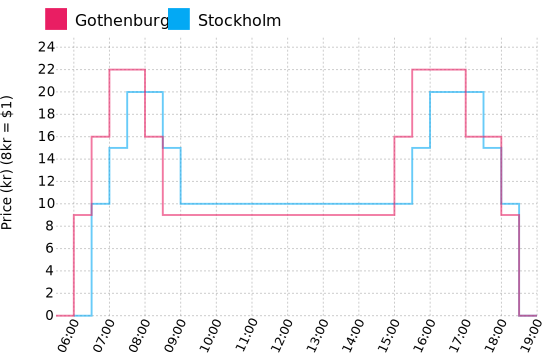
\includegraphics[width=5in]{../img/sweden-prices.png}
\caption{Sweden price structure \citep{transportstyrelsen2015}}
\label{fig:sweden-schedules}
\end{figure}

\subsection{Results}

The Tax has cut both traffic flow and travel times. Traversals of the cordon have fallen by 20-21\%. This figure was in excess of the forecast 16\% fall, due to the fact off-peak travel fell by almost the same amount (21\%) as peak travel (20\%) \citep{Eliasson2013}. Models had predicted off-peak travel would fall only 14\% due to lower mid-day charges. The fall in person-trips was similar for commuters (24\%) and discretionary travelers (22\%), but the two groups adapted differently: commuters who stopped driving switched to public transit, while discretionary travelers cancelled or rerouted their trips \citep{FranklinEtAl2010}. \citet{Eliasson2013} estimate that the Tax raised public transit ridership 4-5\%, or 8-10 thousand riders per day, and that vehicle-kilometers-traveled within the zone fell 10-15 percent. \citet{Karlstrom2009} find only weak evidence of departure time rescheduling.

\subsection{Finances}
Costs due to delays 600 MSEK \citet[p. 843]{GullbergIsaksson2009}.

Congestion Tax not so different than the gasoline tax, which is collected and then redistributed.
\section{Milan Ecopass and Area C}\label{sec:milan}

\subsection{Implementation}

To frame the the Milan experience requires two pieces of context.\footnote{This history is based on \citet{Mattioli2012}, with support from \citep{Rotaris2010}.} First, Italian cities commonly operate ``limited traffic zones'' (ZTL's), areas where vehicle access is restricted. A ZTL, for instance, might ban private vehicles during the workday except for residents. Milan already had a camera-enforced ZTL inside its Cherchia dei Bastioni (CB)---a ring of 16th century fortifications around the city center where about 80,000 people live---so charging required little new infrastructure. Second, Milan has relatively high use of cars and motorcycles---especially those with diesel engines---and is located in the relatively windless Po Valley. The combination of geography and vehicle use has begotten severe particulate matter pollution, leading to constant violation of European Union directives on air quality. Thus, while other cities have touted their schemes' environmental impacts, Milan is the only city which has explicitly designed a DCP scheme to combat air pollution.

 Letizia Moratti proposed charging for access to the CB following her election as Mayor of Milan in 2006. On January 1, 2008 launch of ``Ecopass,'' an ANPR-enforced daily license (one charge pays for unlimited travel). Ecopass had a complex charging structure (see Table \ref{tab:milan-ecopass-prices}) and liberal exemptions---especially green vehicles. Thus, the share of chargeable vehicles entering the zone fell sharply in the first few years. Observers believed Ecopass was not having its advertised effect, particularly since air pollution worsed in early 2010. Consequently, in 2010 activists organized a petition drive for a number of environmental and transportation referenda, including one to extend road pricing to all cars and to extend the charging area. In the July 2011 referendum, all the proposed measures passwed, including the Ecopass proposal with 79 percent of votes cast. Around the same time, Moratti was replaced as mayor by Giuliano Pisapia, who set about remaking Ecopass. The reorganized system, rebranded ``Area C,'' commenced operation on January 16, 2012. Area C does not have a larger charging zone, but it does charge more vehicles.

\subsection{Design}

The charging zone of both Area C and Ecopass is an 8 km$^{2}$ area of central Milan called the Cerchia dei Bastioni (CB) (see Figure \ref{fig:milan-map}). The cordon consists of 43 access points where cameras read the number plates of vehicles entering (but not exiting). Like the LCC, charges are flat over the day; they are in force from 7:30 AM to 7:30 PM on weekdays, except that since September 2012 Area C stops charging at 6 PM on Thursdays in order to promote a night of shopping and cultural events \citep{CorriereDellaSera2012}. 

The standard way to pay is to buy a digital ``ticket'' at banks, parking meters, online, ATM's or in stores and then ``activate it''---that is, associate it with a plate number on a particular day---by phone, SMS, online or at municipal offices. One has until midnight until the day after entry to pay, although it is also possible to pay in advance. Since the switch to Area C, users can also sign up for a Telepass radio-frequency transponder to pay by debit automatically. 

What most distinguishes Ecopass from Area C is the charging structure: Ecopass involved a schedule of five emission classes, while Area C involves three user classes: resident, ``service vehicle'' and standard. See Tables \ref{tab:milan-ecopass-prices} and \ref{tab:milan-area-c-prices}. ``Service'' vehicles are mostly commercial vehicles for delivery and construction, as defined according to complex rules which change over time. 

Both systems have many exemptions and caveats. Motorcycles and scooters, electric vehicles, certain green vehicles, taxis, public buses and certain emergency or government vehicles have been exempt under both schemes. Instead of Ecopass' sliding scale, Area C simply bans most high emission vehicles and vehicles longer than 7.5 meters, with some exceptions, while exempting a changing number of green vehicles. The list of exemptions and prohibitions changes from time to time: for instance, in February 2017 LPG and CNG vehicles lost their exempt status, while certain diesel vehicles were banned. Ecopass offered residents of the CB a 50\% discount on their first 50 entries per year and a 40\% discount on the next fifty; but under Area C residents receive 40 free days per year and thereafter pay the \euro 2 residents rate. Since late 2012, the standard charge is only \euro3 for vehicles which park for four or more hours at a garage participating in an agreement with the city government. Finally, Ecopass lets certain licensed buses for tourists and students that longer than 7.5m can enter the CB subject to a scale that slides up to \euro 100 with the size of the vehicle.

\begin{figure}[ht]
	\includegraphics[width=.8\textwidth]{../img/milan-map.jpg}
	\caption{Milan Ecopass/Area C \citep{Rotaris2010}}
	\label{fig:milan-map}
\end{figure}

\begin{table}
\begin{center}
\begin{tabular}{|>{\centering}m{1.8cm}|>{\centering}m{1.8cm}|>{\centering}p{1.8cm}|}
\hline 
Emissions Class & Charge (\euro) \tabularnewline
\hline 
\hline 
1 & 0 \tabularnewline
\hline 
2 & 0 \tabularnewline
\hline 
3 & 2 \tabularnewline
\hline 
4 & 5 \tabularnewline
\hline 
5 & 10 \tabularnewline
\hline 
\end{tabular}
\par\end{center}
\caption{Ecopass prices. Lower classes are less polluting. Class I includes hybrid and electric cars. Class V low-efficiency diesel and buses. \citep{Rotaris2010} }\label{tab:milan-ecopass-prices}
\end{table}

\begin{table}

\begin{center}
\begin{tabular}{|>{\centering}m{2.2cm}|>{\centering}m{1.8cm}|}
\hline 
User Class & Charge (\euro)\tabularnewline
\hline 
\hline 
standard & 5\tabularnewline
\hline 
residents & 2\tabularnewline
\hline 
service vehicle & 3\tabularnewline
\hline 
\end{tabular}
\par\end{center}
\caption{Area C prices. ``Service vehicles'' are those enaged in certain commercial activities.}\label{tab:milan-area-c-prices}
\end{table}

\subsection{Transportation impacts}

Milan has the smallest literature of any of the schemes we visit. Still, the city has collected a great deal of data on traffic flow and emissions and has published annual reports on both Ecopass and Area C's impacts.\footnote{http://www.comune.milano.it/wps/portal/ist/it/servizi/mobilita/Area\_C/motivazioni}  

In the first year of Ecopass, entries to the CB during charging hours fell 14.6\% \citep[Tab. 2, p. 145]{Croci2015}. From 2008 to 2011, traffic recomposed quickly: in 2008, 22\% of entering vehicles paid the toll, but by 2011 the share had fallen to 14.1\%. See Fig. XXX for the trend of paying vs exempt traffic from Jan. 2008 to June 2010. The number of vehicles in the most polluting classes (classes 3-5 of Tab. \ref{tab:milan-ecopass-prices}) fell 70\%.

The switch to Area C coincided with a further reduction in entries which has been sustained (see Fig. \ref{fig:milan-entries}). The charged share has risen substantially: in 2016, 56\% of vehicles are subject to charge---four times the 14.1\% observed under Ecopass \citep[p. 13]{AMAT2017}.

Comparisons of private vehicle speeds seem only to be reported for the first year of Ecopass, when speed in the CB rose 4\% during the morning rush \citep{AMMA2009}. Public transit speeds increased more, but this effect was probably due to new bus lanes.

\begin{figure}[ht]
	\includegraphics[width=\textwidth]{../img/milan-entries2.png}
	\caption{Entries to the Cerchia dei Bastioni. 2011 was the last year of Ecopass; years following are under Area C. \citep[p. 9]{AMAT2017}}
	\label{fig:milan-entries}
\end{figure}

In 2012, protests by owners of parking garages in the CB led to a court-ordered suspension of charging that lasted from from 25 July to September 17; because of its random nature, have used the suspension as an experiment to test the scheme's effects. \citet{Gibson2015} reaches conclusions regarding the effect of Area C on entries and pollution very different from \citet{Percoco2013} and \citet{Percoco2014}, and the studies even seem to have different data. But all three studies agree that Area C encourages the use of motorcycles, which are exempt---a finding that \citet{Percoco2013} says greatly reduces Area C's power to curb pollution.

\subsection{Finances}

\citet{Rotaris2010} say that implementation costs for Ecopass are not available, but were not very high, since Area C used the same infrastructure as the existing ZTL. Operating costs were \euro 6.5M in 2008 \citep[p. 49]{AMMA2009}. Ecopass revenues were \euro 12.6M in 2008 (the first year), but traffic recomposed toward less-taxed or exempt vehicles, and so revenue fell to \euro 9.6M by 2009 \citep[p. 51]{AMAT2010}. 

Area C has proven more profitable. In 2012, Area C earned \euro 20M and cost \euro 7M to operate \citep{Beria2015}. It does not seem that there were implementation costs for switching to Area C.\footnote{\citet{Croci2016} cites operating costs of \euro 14M and implementation costs of Area C, but the source they provide is a URL on the City of Milan website that is now non-functioning, and this seems to contradict other sources from the City of Milan.} Of the \euro 13 M profit, \euro 3 M went to the BikeMi bikeshare program and \euro 10M to public transport. Area C made \euro 28.3M in 2015 \citep[p. 28]{Milan2016} and \euro 32.3 M in 2016 \citep[p. 25]{Milan2017}, but these figures only count toll revenue---not penalties. 

Penalties for non-compliance seem to have been an major source of revenues. No official data on fines are available, but \citet{Rotaris2010} cites informal sources claiming  penalties for Ecopass exceeded tolls. This estimate seems reasonable in light of the fact that, from 2012-2014 (inclusive), Area C earned roughly \euro 60-75 M in penalties, due to unfamiliarity with the system. Penalties declined each of those years, but in February 2017, Area C was altered such that many alternative fuel cars (e.g., LPG and CNG) lost their exemption and several types of diesel vehicle were banned from the charging zone, leading to a surge in penalties as drivers struggled to adapt.


\section{Gothenburg --- Gothenburg Congestion Tax}\label{sec:gothenburg}

\subsection{Implementation}

The genesis of Gothenburg's pricing system lies in the above-mentioned infrastructure agreement between Stockholm and the national government. Previously, most infrastructure projects in Sweden were funded nationally, but the agreement demonstrated a local/national co-financing model \citep{Borjesson2015,Hysing2015b}. In 2008 the government directed the infrastructure administration to prioritize such co-financing when selecting projects for the 2010-2021 transport investment plan. When a draft of the plan came out in spring 2009, leaders from the Gothenburg region lamented that many of their high-priority projects had been left out, and embarked on negotiations with national officials about co-financing these projects. The negotiations proceeded quickly, and in October 2009 the Gothenburg City Council ratified the ``West Swedish Agreement,'' whereby 17 billion SEK in local funds---including 14 billion from road pricing---would be matched one-for-one by national funds. The Agreement included a 20 billion SEK rail tunnel (the ``Western Link''), a road tunnel, bus lanes and a multi-modal bridge. 

Unlike the protracted process behind the Stockholm Congestion tax, the selection of projects and the design of the road pricing scheme were both rushed, so that the projects could be included in the national investment plan that Parliament passed in April 2010. This provoked controversy, and in the September 2010 elections, voters gave several seats on the Gothenburg City Council to a new party, Vägvalet (``Road Selection''), whose sole issue was opposition to road pricing. In 2012, a public petition drive led the council to  place a on-binding referendum on the coming charges on the 2014 election ballot. Nevertheless, the Council pressed ahead, and the Gothenburg Congestion Tax (GCT) launched on January 1st, 2013 with a design copied from the SCT. In September 2014, the referendum result showed 57\% of votes cast were against continuing the charge, but since the referendum was only consultative, the Council decided to keep the Tax in order to fulfill Gothenburg's end of the West Swedish Agreement. This motive has been well illustrated by the decision to increase tolls in January 2015 after early revenues fell short of projections.

\subsection{Design}

Gothenburg's scheme uses the same technology and design as Stockholm's: cameras identify drivers crossing tolling sites in either direction, and tolls vary by time-of-day. Figure \ref{fig:gothenburg-prices} shows the tolling schedule in place today, which is somewhat larger than the original schedule. There is a daily maximum charge of 60 SEK, and the same vehicles are exempt as in Stockholm. Figure \ref{fig:Gothenburg-map} shows the tolling sites form a cordon around downtown Gothenburg, but there are also sites at the \"Alvsborg Bridge (toll site \#11) and along a highway north of the city where congestion would otherwise be severe. Note that more tolling sites are required for Gothenburg than for Stockholm owing to the lack of water boundaries.

Gothenburg has the same exemptions has Stockholm, and the Tax is turned off in July. One feature unique to Gothenburg's scheme is the ``single charge'' or  ``multi-passage'' rule: no matter how many tolling sites a vehicle crosses within 60 minutes, it is charged only once, with the toll being the highest among the possible charges. 

\begin{figure}[ht]
\includegraphics[width=0.7\textwidth]{../img/gburg-map.png}
\caption{Gothenburg Congestion Tax zone \citep{transportstyrelsen2015}\label{fig:Gothenburg-map}}
\end{figure}

\begin{figure}
    \includegraphics[width=0.8\textwidth]{../img/gothenburg-prices.png}
    \caption{Gothenburg price structure } 
    \label{fig:gothenburg-prices}
\end{figure}

\subsection{Transportation impacts}

Between 2012 and 2013, cordon crossings during charging hours fell 12\%, rather than the 15\% forecast by models \citep{Borjesson2015}. Although peak crossings were expected to fall more than off-peak, due to the higher charges, in fact both fell by about 12-13\%. (Recall that Stockholm also surprised observers by showing the same reduction in the peak and off-peak.) Entries have since remained stable \citet[Tab. 5]{Borjesson2018}.

Travel time savings were mild---mostly because Gothenburg was not very congested in the first place. Results appear in Fig. \ref{fig:Gothenburg-travel-times}. Inner arterials are the highways circled in Fig. \ref{fig:Gothenburg-map}; outer arterials are the uncircled highways outside the zone; bypasses are highways further out than the map shows. As the figure shows, congestion intitially was much lighter than it was in Stockholm, and there was very little change in traffic within the cordon. The dramatic reduction on the inner arterials is attenuated by the fact that travel time on these links had only been about 5 minutes during the morning peak \citep{Borjesson2015}.

Surveys conducted before and after charging show that commuters switched to public transport, while discretionary travelers traveled less frequently or switched destinations. Accounting for external factors, the charge is estimated to have raised public transport ridership by about 4.5-6.5\% \citep{Borjesson2015}.

\begin{figure}[ht]
\includegraphics[width=0.55\columnwidth]{../img/gburg-travel-times.png}

\caption{Gothenburg 6-10 A.M. Increase in travel times on selected categories of road relative to free-flow speeds, before (Oct 2012) and after (Oct 2013) the Congestion Tax. \citep{Borjesson2015} \label{fig:Gothenburg-travel-times}}

\end{figure}

Like Stockholm, Gothenburg's experience supports Theme II: the 2015 toll increase resulted in no real change in entries during the peak hours, although the increase was not as substantial as in Stockholm \citep[p. 43, Tab. 6]{Borjesson2018}.

\subsection{Finances}

The GCT cost only 410 MSEK to implement if we count only those costs specific to Gothenburg \citep[p. 40]{Borjesson2018}. However, in 2012, Sweden spent 350 MSEK to replace the IT system for the Stockholm Congestion Tax with a national system that Gothenburg and two bridges elsewhere in Sweden could also use; arguably some part of this expense could be attributed to Gothenburg. 

In the first year, 2013, the GCT earned 720 MSEK in charges and about 80 MSEK in penalties---short of the amount that had been forecast in 2009 \citep[pp. 142-143]{Borjesson2015}. \citet{Borjesson2015} blame the shortfall on economic factors (fuel prices, recession) and the fact that 45\% of trips into the cordon during charging hours took advantage of the ``multi-passage'' rule---rather than the 30\% analysts predicted. The shortfall is what led authorities to raise the toll in 2015, since---unlike in London where revenues are hypothecated to transit in a vague way---the Western Swedish Agreement commits Gothenburg to pay for specific projects. The increase led revenues to jump from 80 MSEK in 2014 to 99.5 million EUR in 2015. Operating costs have been around 130 MSEK per year and are declining \citep[table 3]{Borjesson2018}.





\section{The future}\label{sec:future}

The story of DCP is certainly unfinished. There are now several important developments underway, including revamping of extant schemes and the possible implementation of new ones.

The most likely source of major developments is Singapore. Singapore has already started the process of changing ERP into ERP 2.0, a distance-based charge, administered by satellite tracking and roadside cameras.\footnote{http://www.straitstimes.com/singapore/transport/erp-20-goes-the-distance-with-new-tech} The new system is planned to launch in 2020, and will also incorporate parking charges.

In London, the LCC infrastructure is being purposed for pollution control. On October 23, 2017, TfL commenced operation of the ``T-charge'' system. This scheme charges an additional \pounds 10 to older vehicles with higher emissions to enter the CZ during the same charging period as the LCC.\footnote{ ``T-Charge: New London traffic charge comes into force'' http://www.bbc.com/news/uk-england-london-41695116} The measure is a step on the way to the April 2019 implementation of an ``Ultra-Low Emission Zone,'' which would enact much higher charges (e.g., up to \pounds 100 for certain trucks) on a broader range of vehicles than the T-Charge (including motorcycles) and apply 24 hours every day of the year.\footnote{``Ultra Low Emission Zone'' https://tfl.gov.uk/modes/driving/ultra-low-emission-zone} London Mayor Sadiq Kahn has also entertained the idea of replacing the LCC with a distance-based charge.\footnote{https://www.citylab.com/transportation/2017/06/london-driving-mileage-fee-sadiq-khan/531270/}

The Swedish Ministry of Finance recently proposed to increase the Stockholm Congestion Tax, by 10 SEK at the peaks (28\%), and to extend charging to more days of the year.\footnote{https://mitti.se/nyheter/trafik/forslaget-dyrare-trangselskatt/?omrade=hela-stockholm} The Stockholm government is receptive to the idea as long as revenues are invented in local transportation.

In Vancouver, local governments and the regional transportation authority (TransLink) have established a special commission tasked with researching options for congestion pricing. Their first report, \citep{vancouver2018}, considers---among more traditional scheme designs---implementing DCP using a distance-based charge. 

In Fall of 2017, Andrew Cuomo, governor of the state of New York, appointed a task force called FixNYC to reexamine at DCP for lower Manhattan.\footnote{https://www.nytimes.com/2018/01/16/nyregion/cuomos-congestion-pricing-for-new-york-city-begins-to-take-shape.html} The task force has yet to release a report, but it reportedly will incorporate a cordon toll as well as distance- and time-based levies on taxis and ridesharing vehicles.


% ERP 2.0

% The San Francisco County Transportation Authority is currently running a long-term study 

% SAN FRANSCISCO MAPS STUDY. NEW YORK CITY. VANCOUVER.

\section{Conclusion}\label{sec:conclusion}

This paper has reviewed the history of DCP, from its first appearance in the minds of British and American academics in the 1950's to current plans for new and reconfigured systems across the world. Moreover, even among the small number of schemes implemented so far, there is enormous diversity in implementation, design, effects and finances. But experience shows that DCP is effective at reducing entries to tolled zones by charged  trips, raising speeds, raising funds and encouraging people to travel by priveleged modes and vehicles. By way of a conclusion, we now briefly mention some developments omitted for brevity or want of literature and return to the themes proposed in Sec. \ref{ssec:themes}.

\subsection{Themes}

Theme I: exemptions are surprisingly consequential. The ALS, LCC and SCT all saw taxi traffic jump upon implementation. The LCC charging zone has been swamped by exempt private-hire vehicles in recent years, while for the SCT exempt green vehicles rose to 14\% of traffic before having their exemption cancelled. In Gothenburg, use of the ``multi-passage'' rule was underpredicted. In Milan, the chargable share of traffic fell sharply during the Ecopass regime, and exempt traffic rose quickly, while Area C seems to have encouraged the use of motorcycles. The apparent lesson of Theme I is that cities should be cautious about handing out exemptions. Rather than exempting green vehicles, for instance, a city might do better to ban or charge high-emission vehicles---as London and Milan do explicitly and Singapore does indirectly (by charging larger vehicles more).

Theme II: the fact of a toll is much more consequential than differences in the toll level. The ALS, LCC, SCT and GCT all demonstrated little change in traffic after increasing tolls but dramatic reductions upon introducing tolls, while ERP seems to be an exception and Milan has not increased tolls yet for a particular vehicle class. If true, Theme II has major rammifications for policy. If almost \emph{any} non-zero toll really does dissuade so many drivers, then a city where fairness issues loom large could simply charge low tolls. In particular, if speed in some city responds non-linearly to traffic in-flows, then even a low toll could garner much of the traffic gains of an ``efficient'' toll while imposing less hardship. Of course, choosing low tolls has downsides: the scheme will raise less money and---since large-enough toll increases certainly discourage \emph{some} traffic---permit more congestion.


\pagebreak
\subsection*{References}
\bibliographystyle{apalike}
\bibliography{../../papers/practice,../../papers/theory}

\end{document}